\documentclass{standalone}
\usepackage{tikz}

\def\lw{1.1}
\edef\lwoff{\fpeval{0.5*\lw*sqrt(2)}}
\def\offa{3.1}
\def\offb{6.2}

\begin{document}
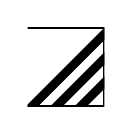
\begin{tikzpicture}[x=1mm,y=1mm,line cap=rect,line width=\lw mm]
\clip (0.25mm,0) rectangle (10,10);
\draw (\lwoff,0)--(10,\fpeval{10-\lwoff}) (\offa+\lwoff,0)--(10,\fpeval{10-\offa-\lwoff}) (\offb+\lwoff,0)--(10,\fpeval{10-\offb-\lwoff});
\draw[line width=0.4mm] (0,0)--(10,0)--(10,10)--(0,10);
\end{tikzpicture}
\end{document}
